\chapter{Ejercicio aspiadora robótica atrapa confeti}\label{chap:aspiradora}
En este capítulo se explica el desarrollo del ejercicio de una aspiradora robótica que atrapa confeti. Por un lado se expone el enunciado y objetivos del ejercicio, por otra parte cómo se ha implementando en la plataforma Kibotics y finalmente una solución de referencia.


\section{Enunciado}
El objetivo de este ejercicio es hacer una aspiradora robótica que se encuentre en una habitación y sea capaz de recoger piezas de confeti cuando ésta pase por encima. Para tener un ejercicio más completo se creará un evaluador automático para contar el confeti recogido en un tiempo determinado.

El alumno deberá programar en Scratch o en Python un algoritmo de planificación de ruta para que la aspiradora consiga atrapar el mayor número de confetis de la habitación en 5 minutos.

\section{Desarrollo del ejercicio}
Para hacer este ejercicio se utilizaron las herramientas Blender, el simulador Websim de Kibotics que contiene la tecnología A-Frame y los lenguajes JavaScript, HTML5 y JSON.

Lo primero que se realizó en este ejercicio fue crear varios prototipos en Blender de una aspiradora robótica. En las Figura 5.1 se puede ver el modelo que se ha creado y utilizado finalmente para el ejercicio.
 
 \begin{figure}[H]
  \begin{subfigure}[b]{0.5\textwidth}
  \centering
    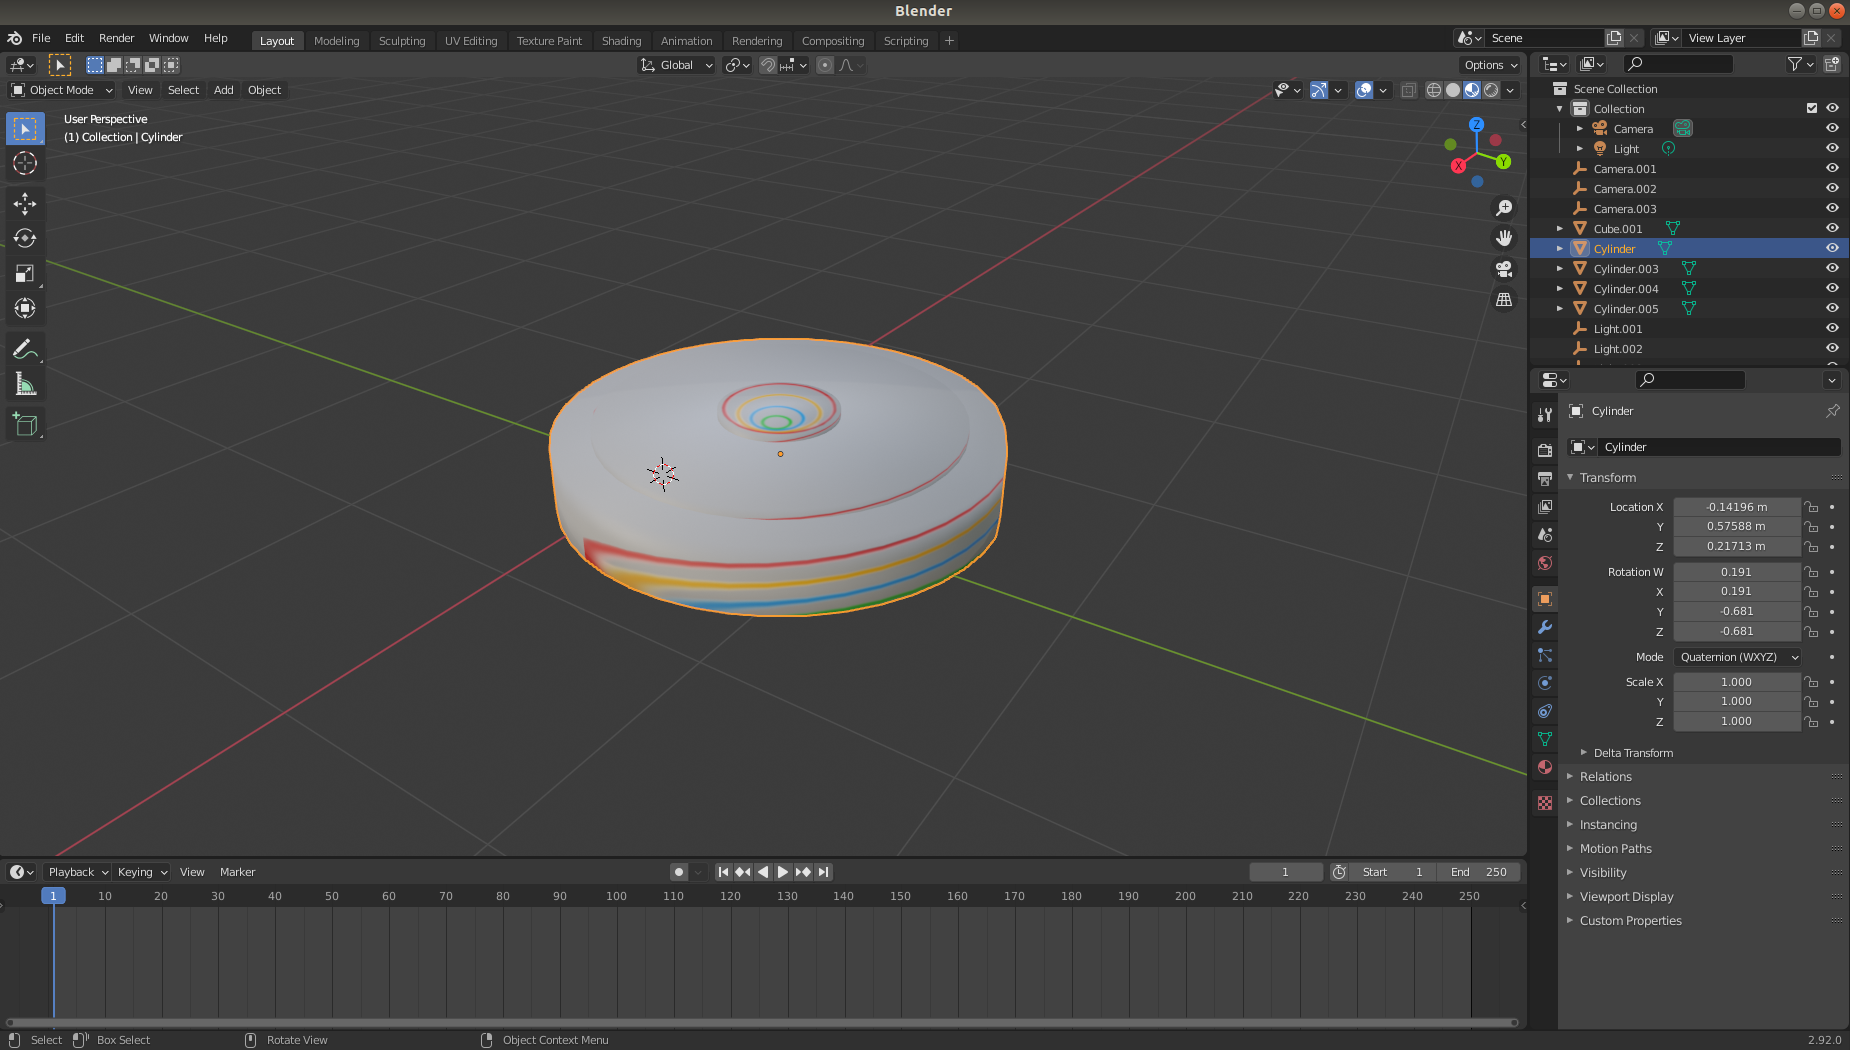
\includegraphics[width=0.95\textwidth, height=0.7\textwidth]{chapters/images/roombablender.png}
    \caption{}
    \label{fig:f1}
  \end{subfigure}
  \hfill
  \begin{subfigure}[b]{0.5\textwidth}
  \centering
    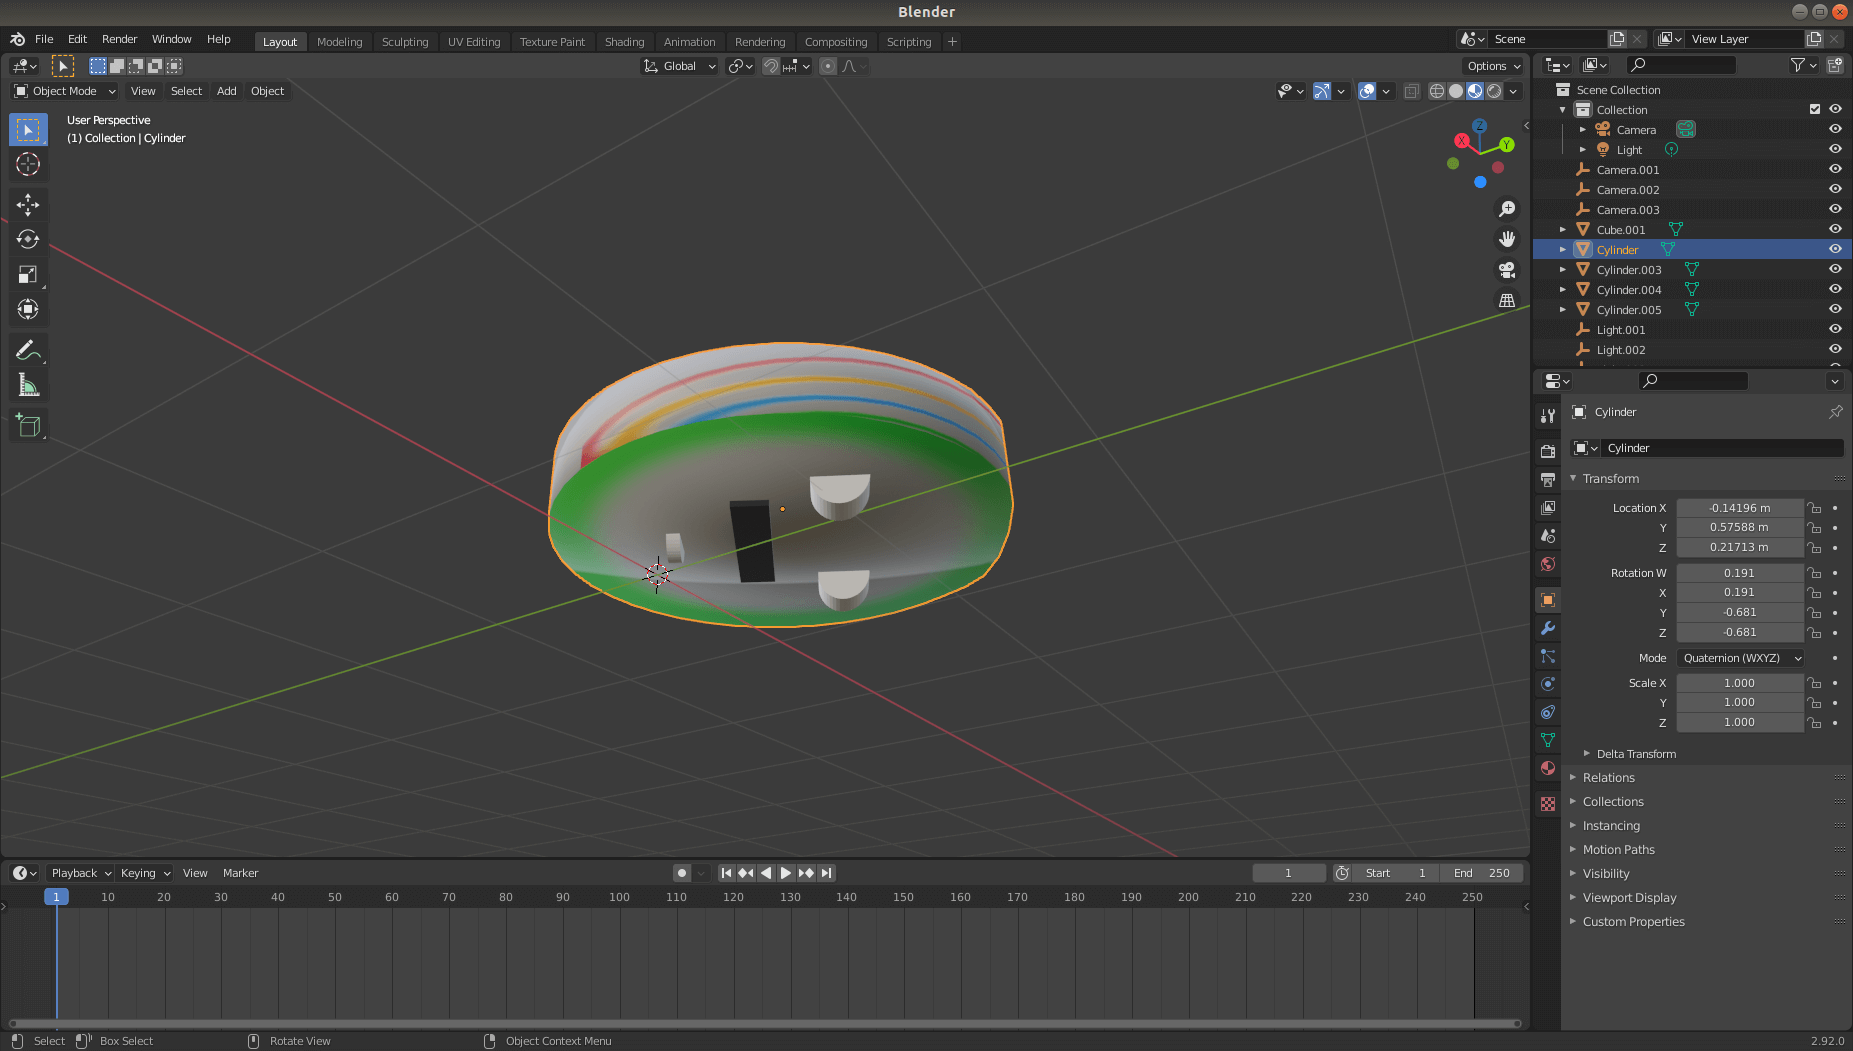
\includegraphics[width=0.95\textwidth, height=0.7\textwidth]{chapters/images/roombablender2.png}
	\caption{}    
    \label{fig:f2}
 
  \end{subfigure}
  \caption{Modelo de la aspiradora robótica  realizado en Blender.}
\end{figure}

A la par se creó el modelo de confeti con la etiqueta \textit{a-cylinder} de A-Frame para hacer pruebas de absorción con código JavaScript.
Las pruebas de absorción se estudiaron tanto en función de la posición como por colisión. En este vídeo \footnote{https://www.youtube.com/watch?v=xkC\_qHXKUDs} se puede ver el primer prototipo con colisión y en este otro  por posición \footnote{https://www.youtube.com/watch?v=If2XMcr1ci4}, al ser un efecto más parecido a lo que ocurre en la realidad se eligió la absorción basada en posición (ver Figura 5.2).

    
\begin{figure}[H]
  \begin{subfigure}[b]{0.5\textwidth}
  \centering
    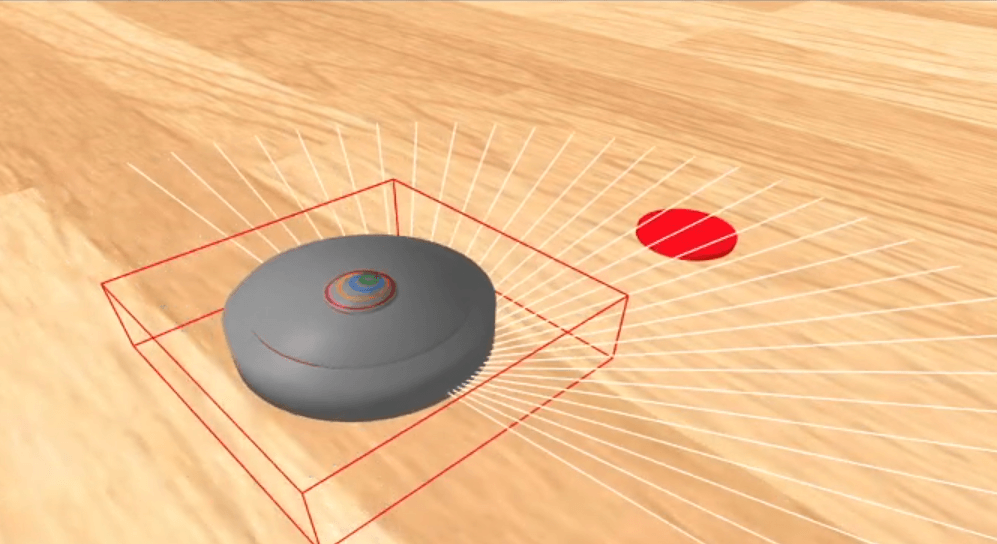
\includegraphics[width=0.8\textwidth, height=0.5\textwidth]{chapters/images/prototiporoomba.png}
    \caption{Modelos aspiradora y confeti en A-Frame}
    \label{fig:f1}
  \end{subfigure}
  \hfill
  \begin{subfigure}[b]{0.5\textwidth}
  \centering
    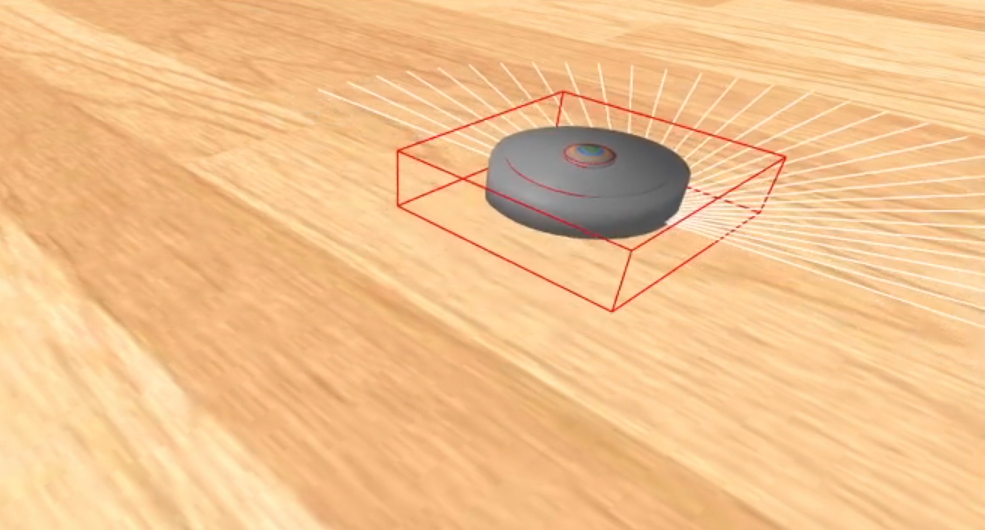
\includegraphics[width=0.8\textwidth, height=0.5\textwidth]{chapters/images/prototiporoomba2.png}
	\caption{Confeti invisible}    
    \label{fig:f2}
 
  \end{subfigure}
  \caption{Absorción por posición, el confeti es invisble cuando el robot pasa por encima.}
\end{figure}

El simulador Websim analiza (\textit{parsea}) ficheros JSON para formar mundos con la tecnología A-Frame. De esta forma es sencillo crear los objetos con pares \textit{``atributo":valor}. A continuación podemos ver cómo se define el id robot del nuevo robot, se importa el gltf-model que hemos creado en Blender de la aspiradora, y se le asignan otros atributos como la posición, escala y rotación del robot. El \textit{dynamic-body} nos facilita el movimiento del robot y el atributo \textit{collide} asigna una malla de colisión para que la aspiradora pueda chocarse con los demás elementos del mundo usando físicas de A-Frame y todo sea mucho más realista.

\begin{lstlisting}
   [...]
        {
            "tag": "a-robot",
            "attr": {
                "id": "a-pibot",
                "gltf-model":"/static/websim/assets/models/roombajderbotgrey.gltf",
                "scale": { "x":2, "y":2, "z":2},
                "position": { "x":0, "y":4, "z":30},
                "rotation": { "x":0, "y":90, "z":0},
                "dynamic-body":{"mass": 10},
                [...]
                "collide":{}

            },
           
  [...]
\end{lstlisting}

El confeti no se crea desde el fichero de configuración dado que se tendrían que crear uno a uno y esto extendería demasiado el fichero. Lo que se ha hecho es que, una vez esta cargado el mundo en el navegador del usuario, usando JavaScript, creamos dinámicamente todos los confetis.

Para hacerlo de esta forma, primero se generó un programa para fijar aleatoriamente las posiciones de los confetis en el mundo, así los confetis quedan esparcidos por la habitación y todos los alumnos cuentan con el mismo escenario. Estas posiciones x, y, z de los confetis se guardaron en otro fichero JSON llamado \textit{data.json}. En total el escenario está formado por 100 confetis de colores. El color de cada confeti se elige aleatoriamente cuando se crean desde JavaScript .

Para leer \textit{data.json} se utiliza
\begin{lstlisting}
 <script type="text/javascript" src="{\% static '/data.json' \%}"></script > 
 \end{lstlisting}
en la plantilla HTML del ejercicio.

\begin{lstlisting}

function getRandomColor() {
    var letters = '0123456789ABCDEF';
    var color = '#';
    for (var i = 0; i < 6; i++) {
      color += letters[Math.floor(Math.random() * 16)];
    }
    return color;
}

document.addEventListener('robot-loaded', (evt)=>{
    localRobot = evt.detail;
    console.log(localRobot);

    var sceneEl = document.querySelector('a-scene');

    // CREATE CONFETI
    var n = 0;
    var n_confetis = 99;
    score = 0;
    var array = JSON.parse(data);

    for ( n = 0; n <=n_confetis ; n++) {
      var c = document.createElement('a-cylinder');
      var num_conf="confeti"+ String(n)
      c.setAttribute('id', num_conf);
      pos = {x:array[n].x, y:0,z:array[n].z}
    
      c.setAttribute('position',pos);
    
      var color = getRandomColor();
      c.setAttribute('color', color);
      c.setAttribute('height', "0.25");
      c.setAttribute('radius', 1);
      sceneEl.appendChild(c);
}
\end{lstlisting}

En el código anterior podemos ver cómo se crea el confeti con a-cylinder. El id es confeti más un número  n, que es un número de 0-99 que se le asigna para crear 100 confetis diferentes (Ejemplo del id del confeti número 50   id=``confeti50"). Además se le asigna los atributos posición con las posiciones que se leen del \textit{data.json} y el color aleatorio, como es un cilindro, se define la altura y radio del confeti.
Los confetis no cuentan con malla de colisión para que el aspirador pueda pasar por encima de ellos y absorberlos de una forma más natural.

La absorción se implementó en JavaScript. Se utilizó la función setInterval que ejecuta las funciones que estén dentro de esta función indefinidamente cada un cierto periodo de tiempo.
Cada 25ms este programa comprueba la distancia entre la aspiradora robótica y cada uno de los confetis. La posición del robot es su centro de masas, por eso se  utilizó la distancia euclídea para calcular la distancia entre el centro del robot y el centro del confeti n, si esta distancia d es menor o igual a 2, el confeti n cambia su atributo 'visible' a false. 

Dentro de la absorción se estableció el evaluador automático. Cada vez que d es menor o igual a 2 se suma un punto e indica que el confeti n ha sido  ``absorbido" por el aspirador. La puntuación máxima es de 100, dado que depende del número de confetis 0-99. También se establece una cuenta atrás de 5:00 minutos y cuando llega a 00:00 se deja de contar y absorber los confetis. Aunque la aspiradora siga pasando por encima de otros confetis que siguen visibles en el escenario, éstos no serán absorbidos ni se aumentará el contador del evaluador.

En este código se puede ver cómo se comprueba las posiciones del confeti para la absorción y la puntuación del evaluador.
\begin{lstlisting}

startEvaluator = () => {
  started = true;
}
roomba=sceneEl.querySelector('#a-pibot')

 setInterval(function(){
       //console.log("Roomba",roomba.getAttribute('position').z);
      // console.log("Confeti",confeti.getAttribute('position'));
       //console.log("Confeti",confeti.getAttribute('position').z)
       for ( n = 0; n <=n_confetis ; n++) {
        d = Math.sqrt(Math.pow((array[n].z-roomba.getAttribute('position').z), 2)+Math.pow((array[n].x-roomba.getAttribute('position').x), 2));

       if ( d <= 2 ){
         num_conf="#confeti"+ String(n)
         confeti=sceneEl.querySelector(num_conf)
         if (confeti.getAttribute('visible') == true) {
	      
	      var counter= document.getElementById('time').innerHTML;
		// Tiempo: 00:00	
	      if((counter[8] =='0') && (counter[9]=='0') && (counter[11]=='0') && (counter[12]== '0')){      
		score = score;
		}else{
		score+=1;
		document.getElementById('confeti_recogido').innerHTML = "Confetti recogido: "+ score;
		}
         }
         confeti.setAttribute('visible', false);
        }
      }
	
    }, 25);
 });
\end{lstlisting}

Una vez se consiguió simular la absorción de los confetis, se mejoró el mundo creando nuevos muebles con Blender (ver Figuras 5.3 y 5.4). De esta forma se mejoró el escenario para que fuera una habitación de una casa (ver Figura 5.5).
\begin{figure}[H]
  \begin{subfigure}[b]{0.5\textwidth}
  \centering
    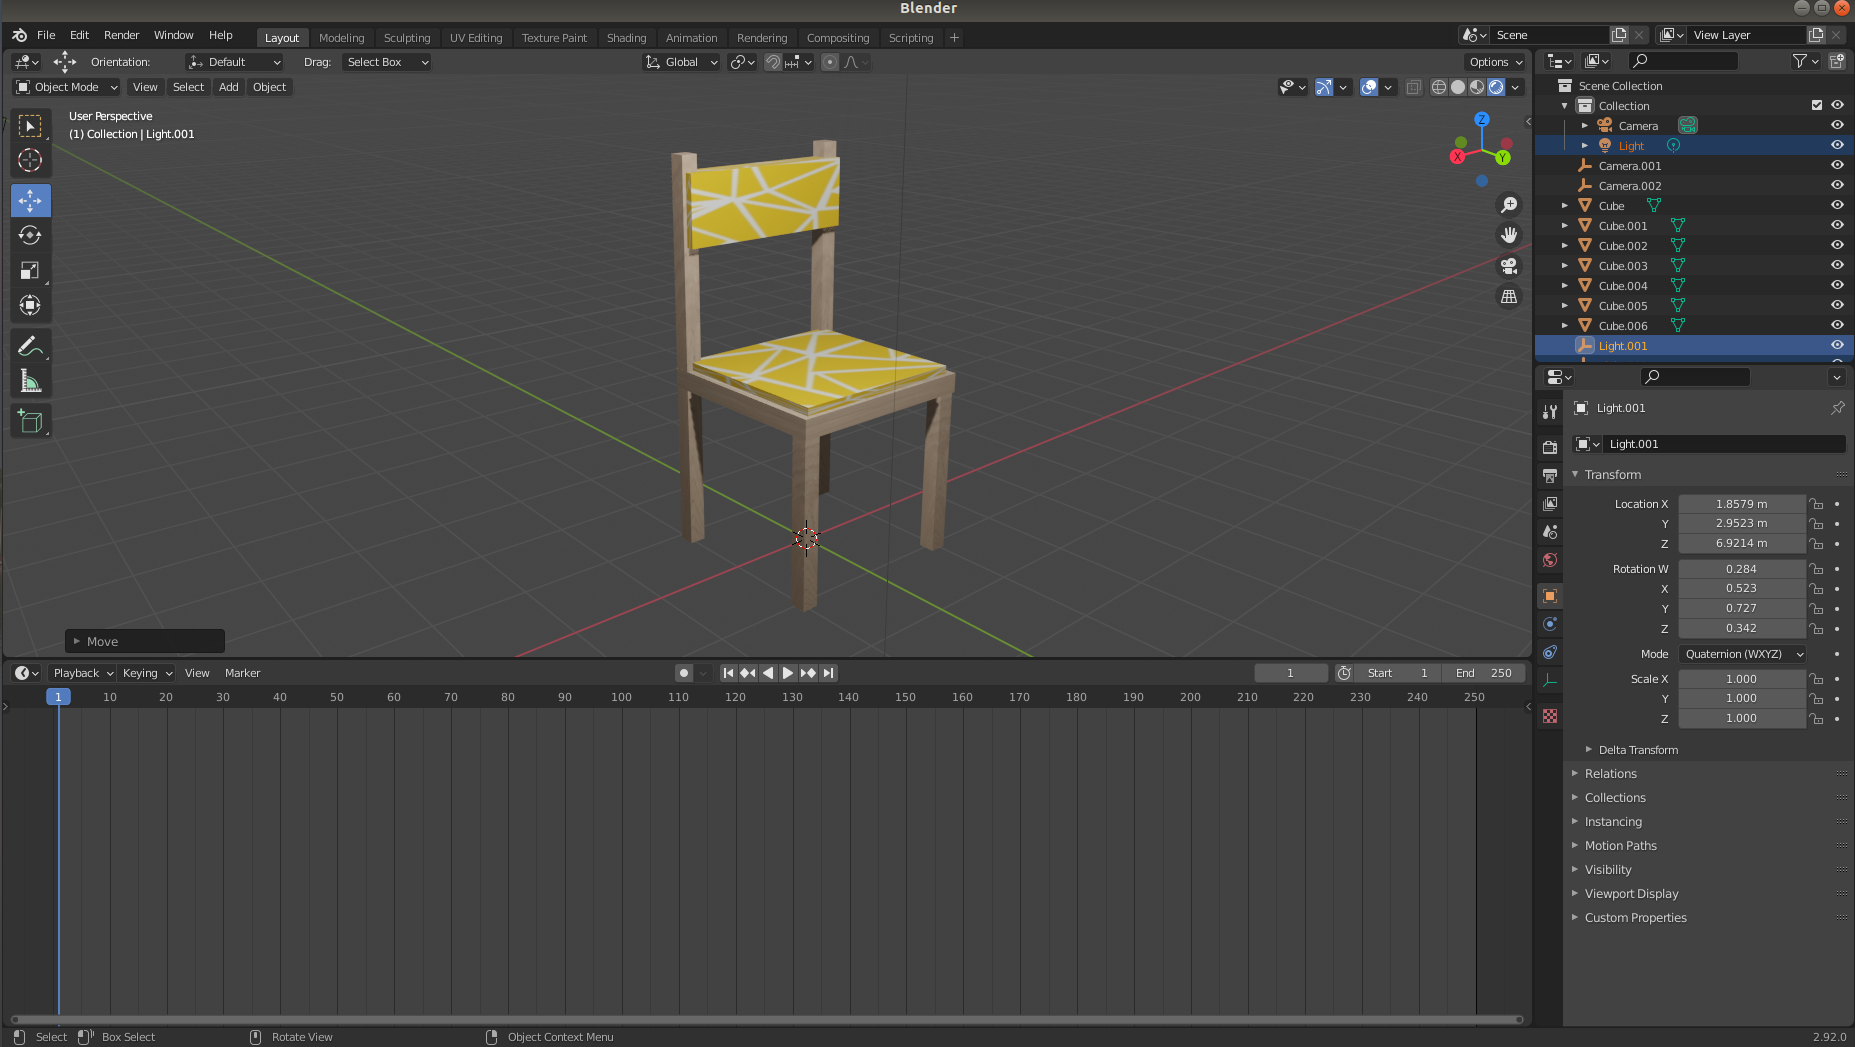
\includegraphics[width=0.95\textwidth, height=0.6\textwidth]{chapters/images/silla.png}
    \caption{Modelo silla}
    \label{fig:f1}
  \end{subfigure}
  \hfill
  \begin{subfigure}[b]{0.5\textwidth}
  \centering
    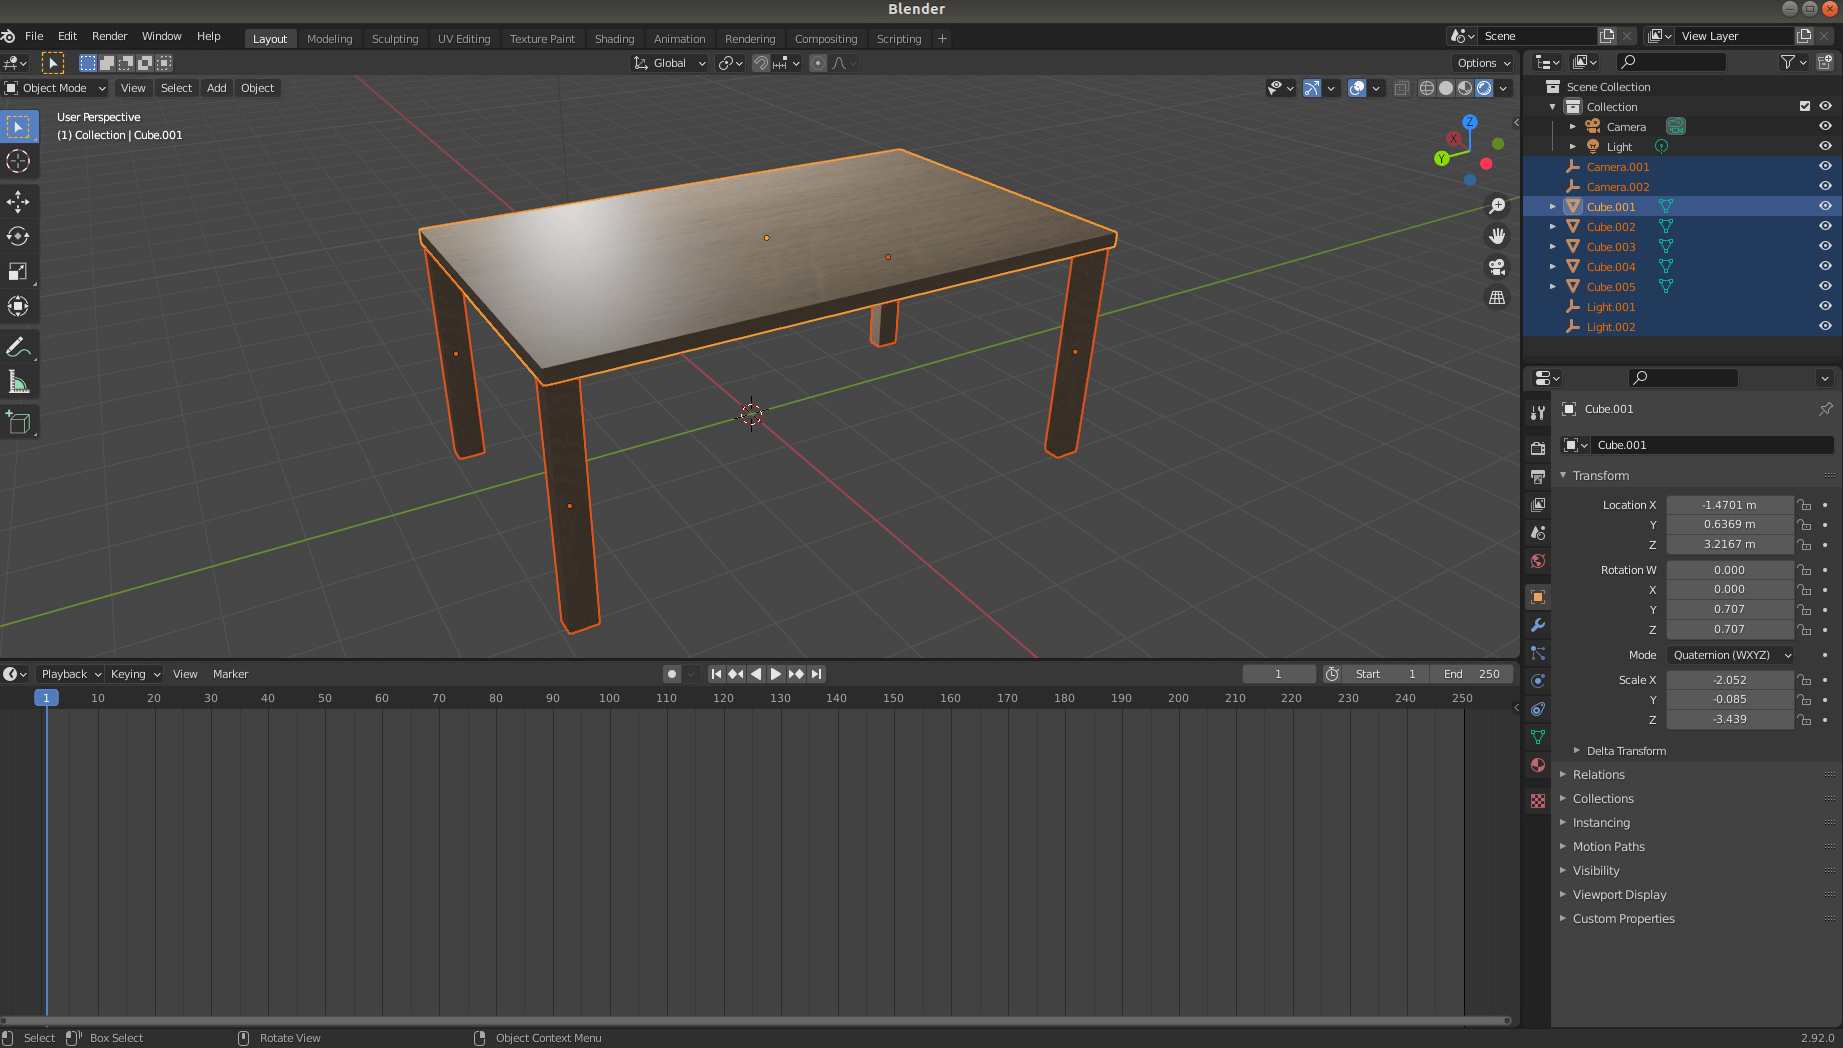
\includegraphics[width=0.95\textwidth, height=0.6\textwidth]{chapters/images/mesa.png}
	\caption{Modelo mesa}    
    \label{fig:f2}
 
  \end{subfigure}
  \caption{Modelos en Blender}
\end{figure}

\begin{figure}[H]
  \centering
 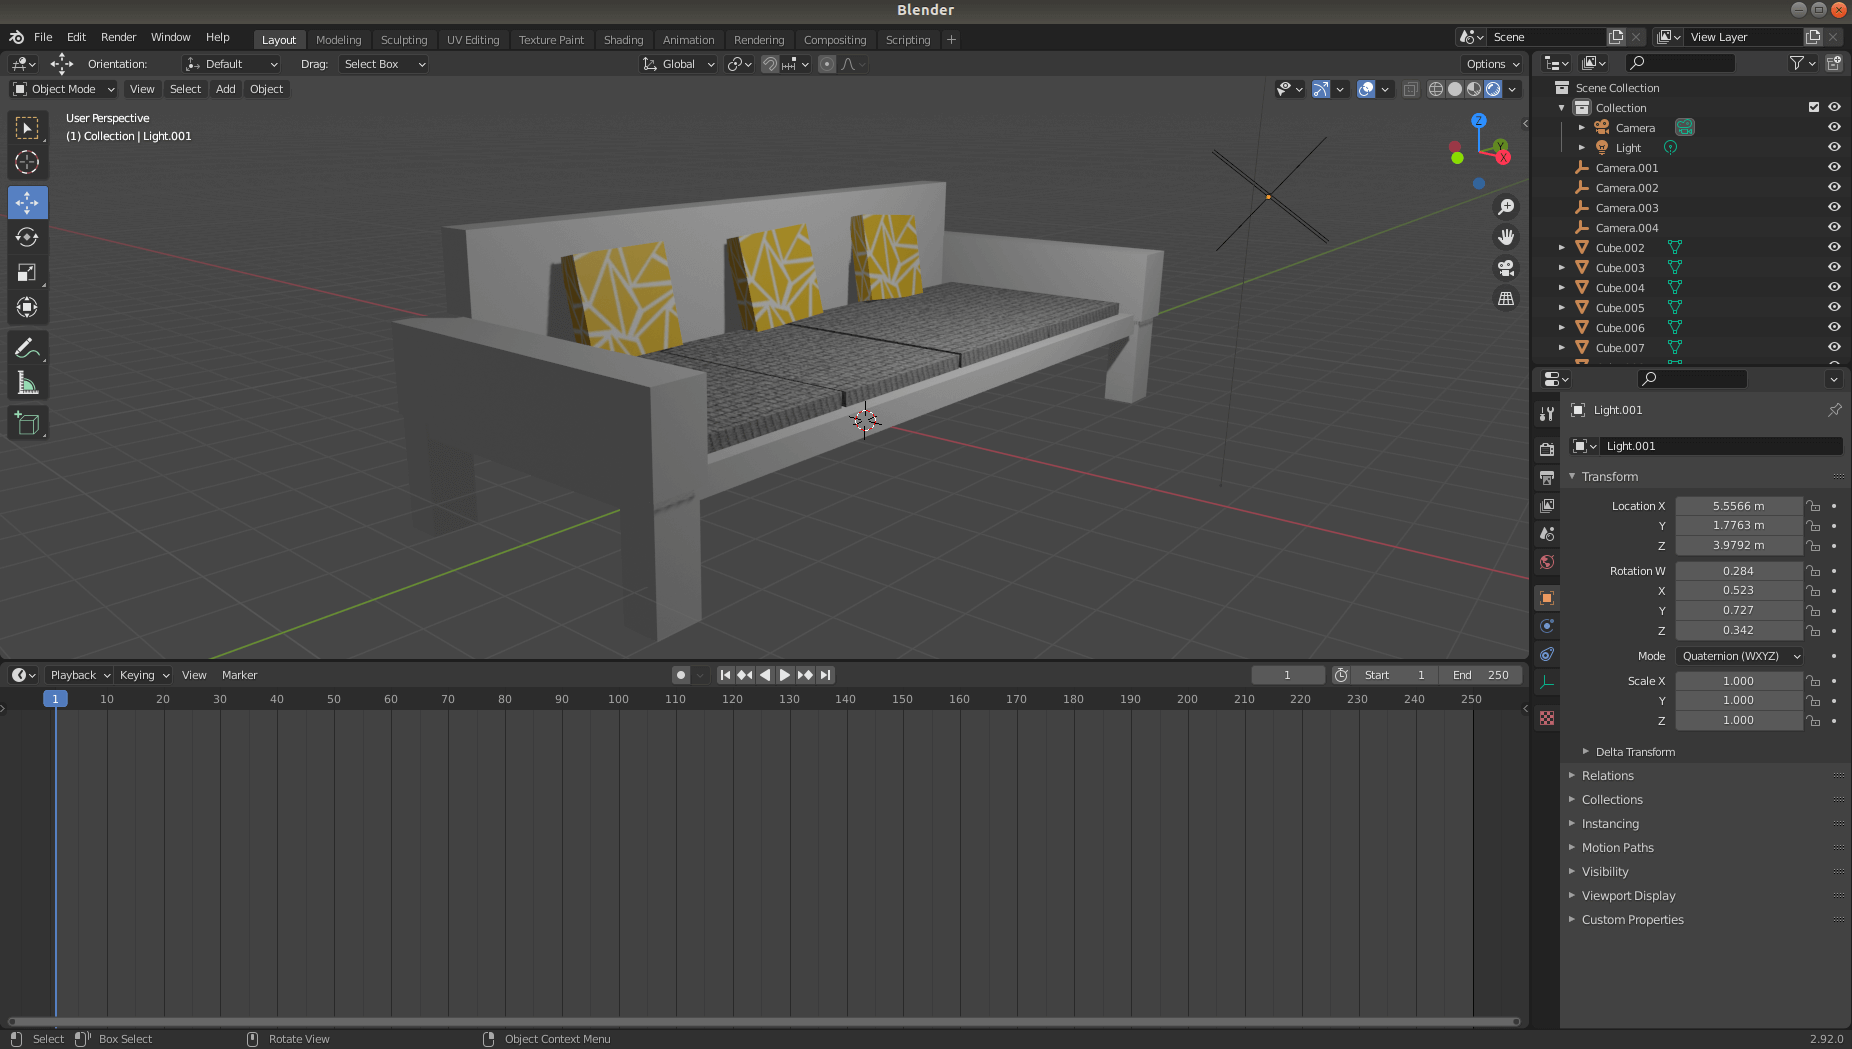
\includegraphics[width=0.9\textwidth, height=0.5\textwidth]{chapters/images/sofa.png}
  \caption{Modelo sofá en Blender}
\end{figure}



\begin{figure}[H]
\centering
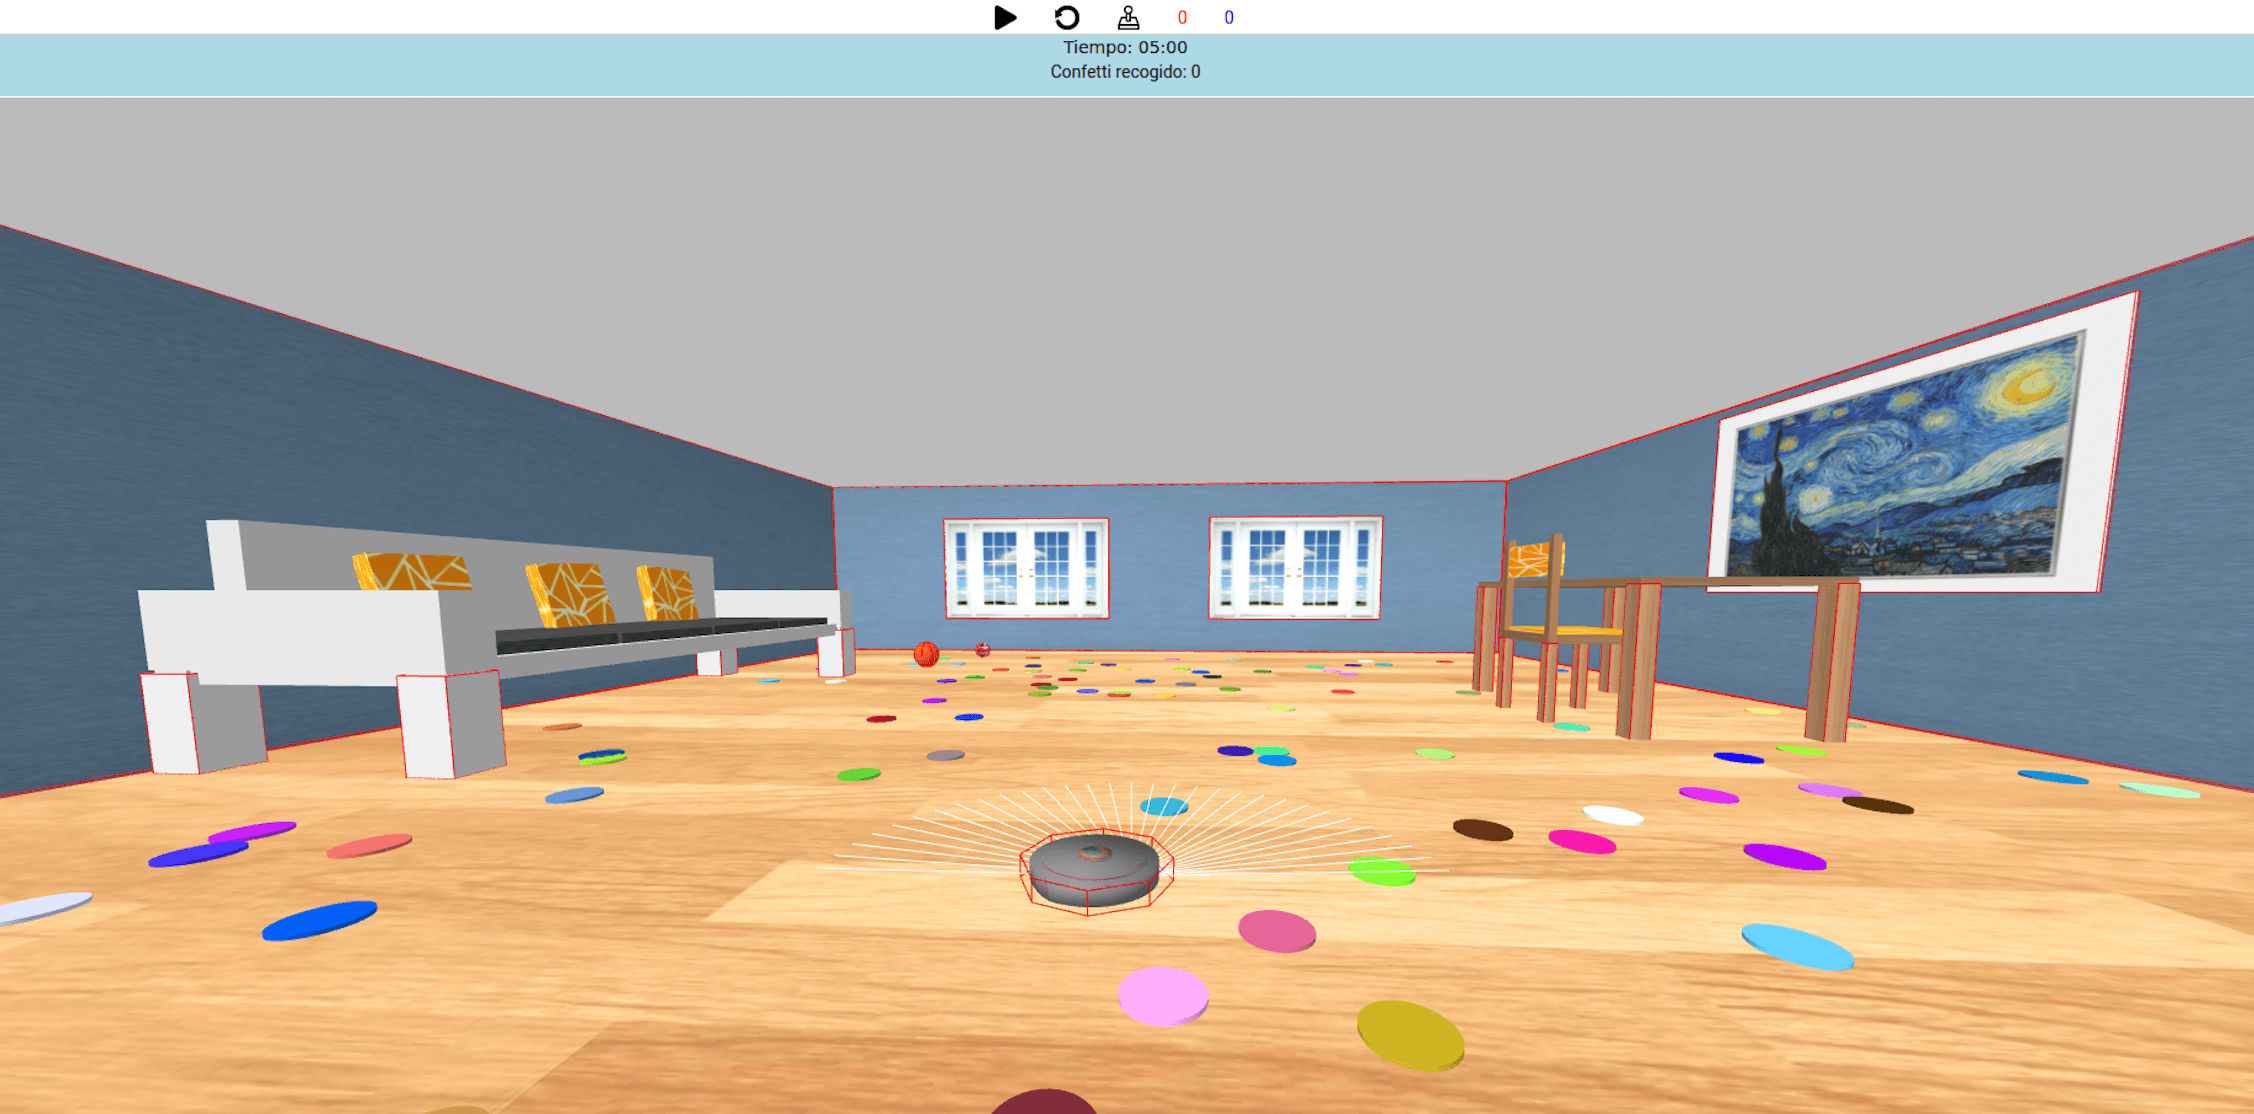
\includegraphics[width=0.8\textwidth, height=0.4\textwidth]{chapters/images/habitacioncon.png}
\caption{Habitación amueblada}
\end{figure}

Para que el escenario tenga mayor dificultad se introdujeron 2 pelotas con movimiento. Para conseguir el movimiento de los objetos había dos posibilidades: animación desde Blender o Animación desde A-Frame. 
Se estudiaron ambas opciones. En el vídeo \footnote{https://www.youtube.com/watch?v=1JPb3Mw8638}  se puede ver cómo hacer una animación no lineal sencilla en Blender para poder usarla en Websim. Se optó por la animación en A-Frame desde el fichero de configuración que era el método ideal para Websim, de esta forma dejamos toda la creación de las pelotas, asignación de texturas, posición y  animación definido en la configuración.

Para animar un objeto desde A-Frame añadimos el atributo \textit{animation} y completamos los valores que sean necesarios como desde dónde a dónde quieres que se mueva  el objeto o el tiempo que quieres que tarde en hacer esa animación. Las dos pelotas tienen estos atributos pero con sus respectivos valores, por ejemplo este código define la animación en diagonal de la pelota de baloncesto: 
\begin{lstlisting}
"animation":{"property: position; from: -40 1.5 -40 ;to: 40 1.5 40; dir: alternate; dur: 10000; loop: true"}
\end{lstlisting}

Finalmente se creó la página web de teoría del ejercicio en HTML5 y se modificaron las plantillas que utiliza el servidor de Kibotics para ver el ejercicio. Este ejercicio se planteó como un juego sencillo en el que se tiene que hacer un algoritmo de planificación de ruta utilizando los sensores y actuadores del robot  para que cuando detecte un objeto próximo, se mueva en ángulos aleatorios. 
En la teoría se explica el objetivo del ejercicio, los requisitos (Figura 5.6), un poco de teoría para explicar al alumno los diferentes algoritmos de cobertura que puede utilizar un aspirador robótico (Figura  5.7) , unas pequeñas pistas y un ¿Sabías que...? (Figura 5.8) hablando de las primeras aspiradoras y como funcionaban. 


\begin{figure}[H]
    \centering
    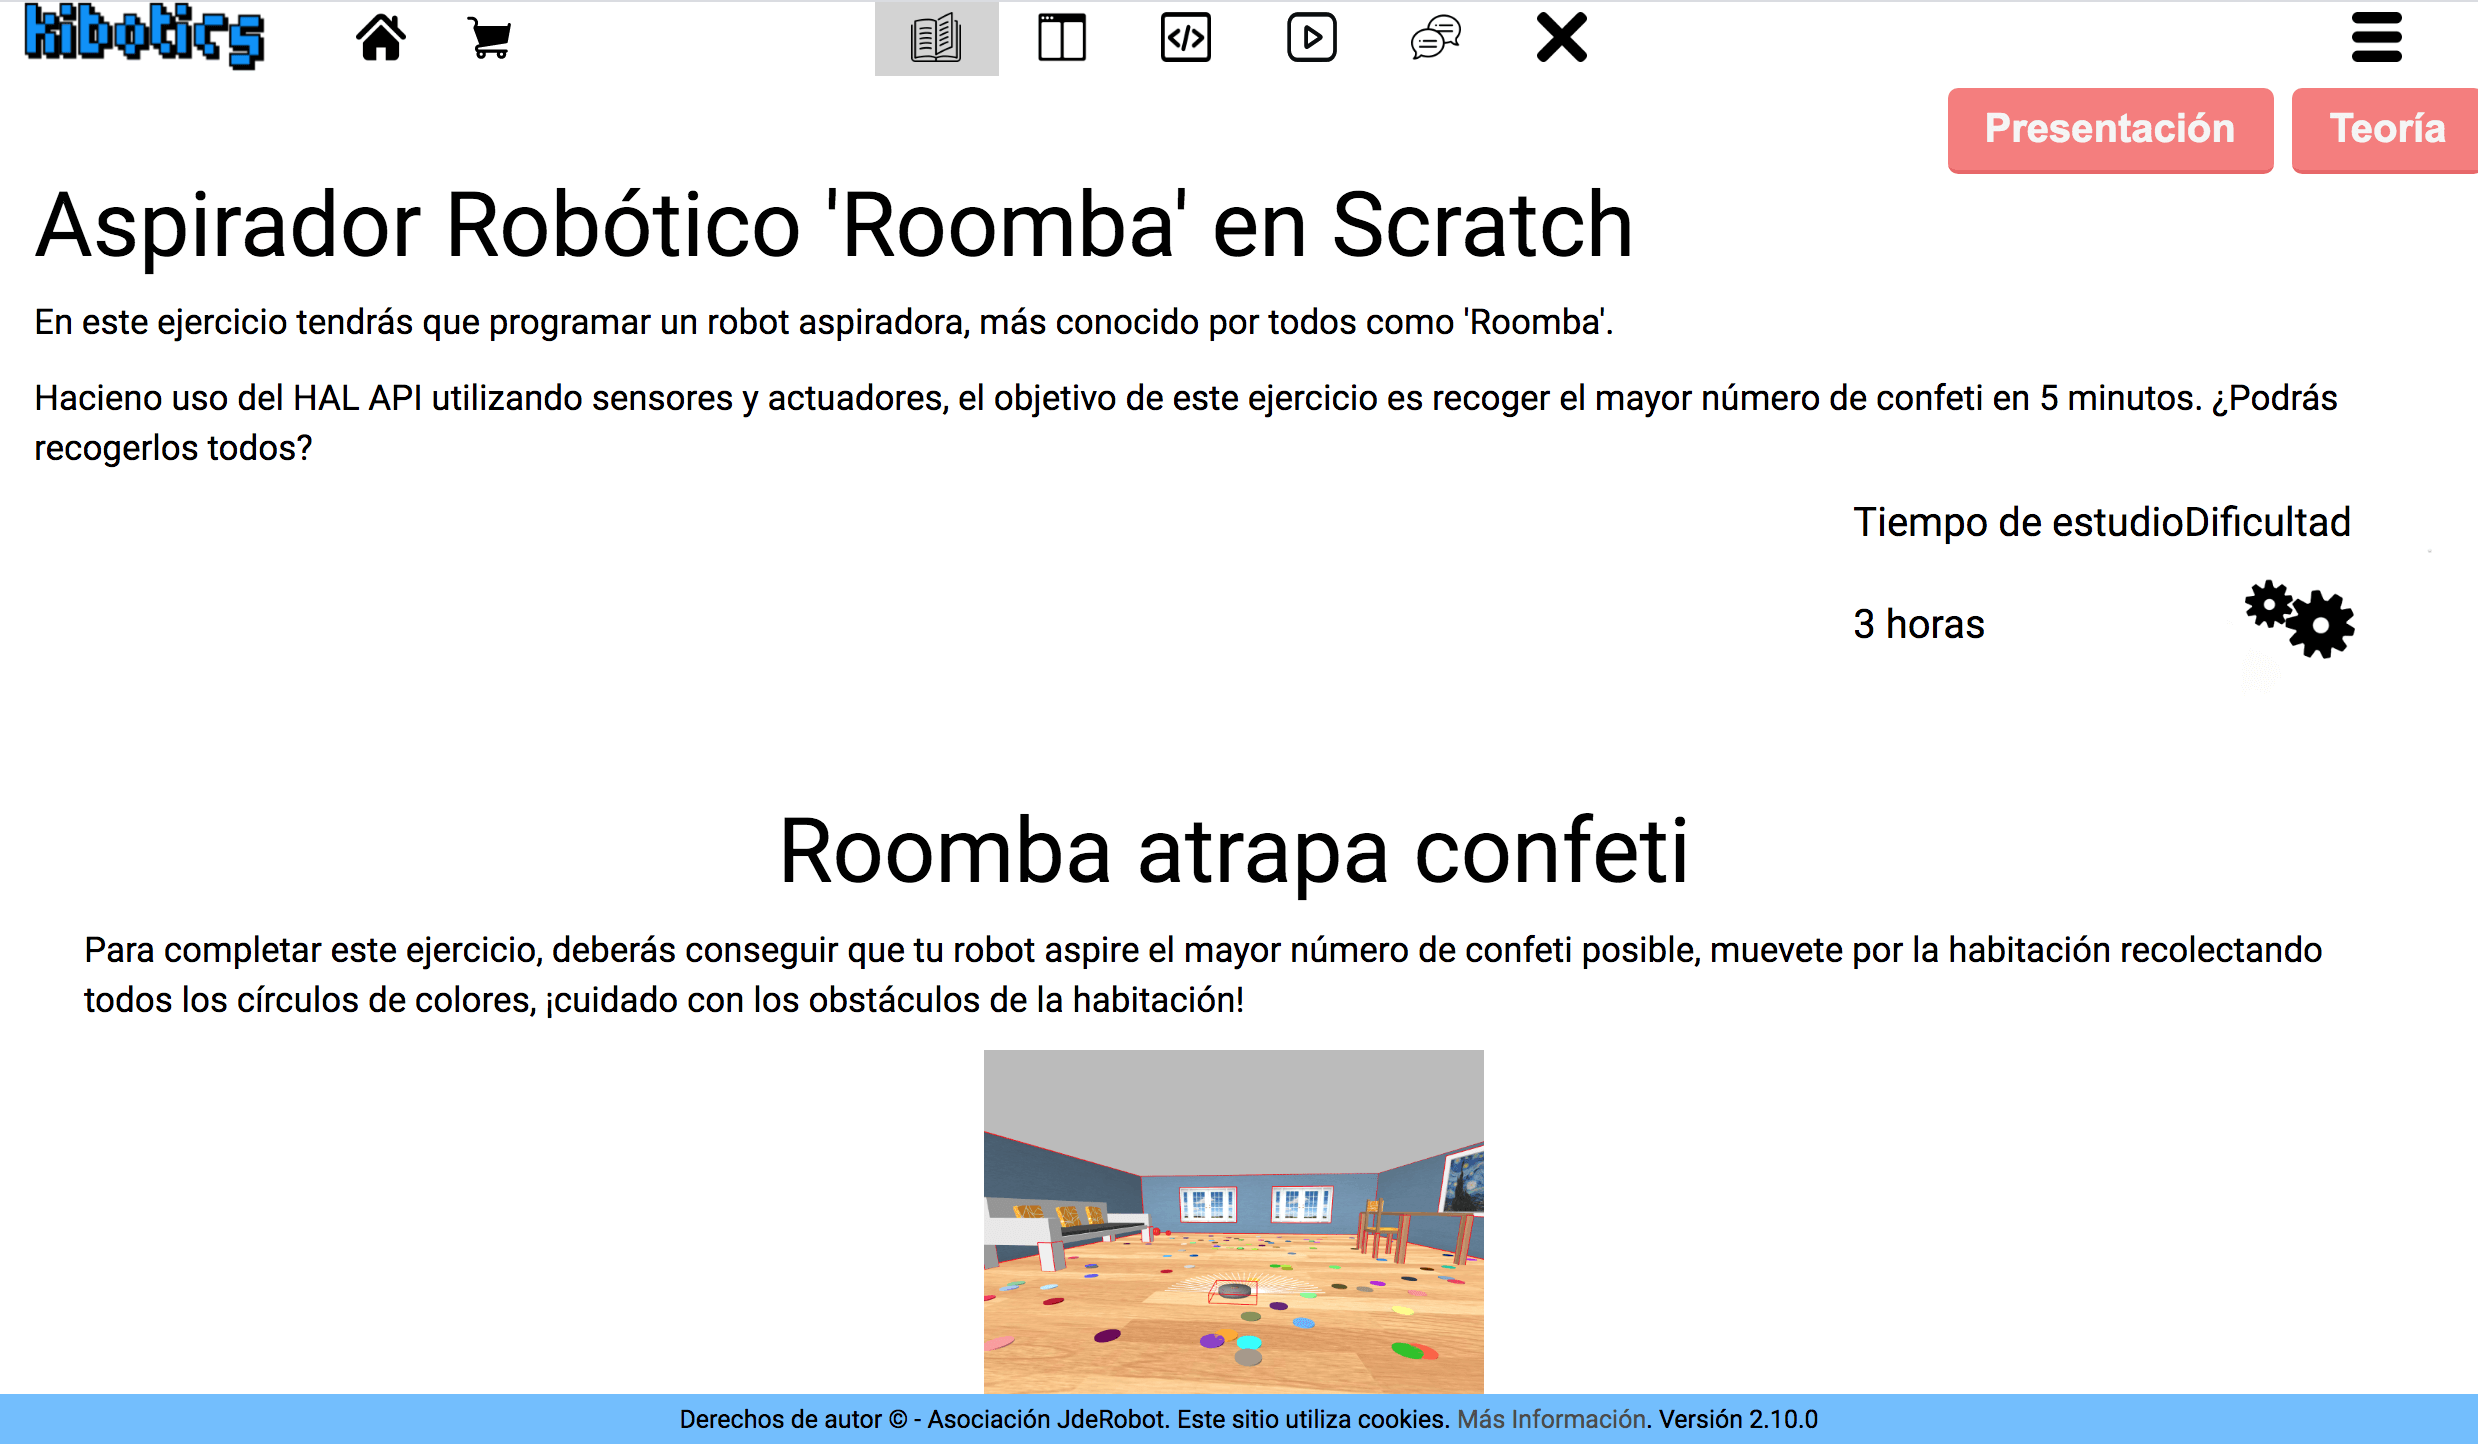
\includegraphics[width=0.8\textwidth, height=0.4\textwidth]{chapters/images/teoria1.png}
    \caption{Página de teoría enunciado y requisitos}
    \label{fig:my_label}
\end{figure}
\begin{figure}[H]
    \centering
    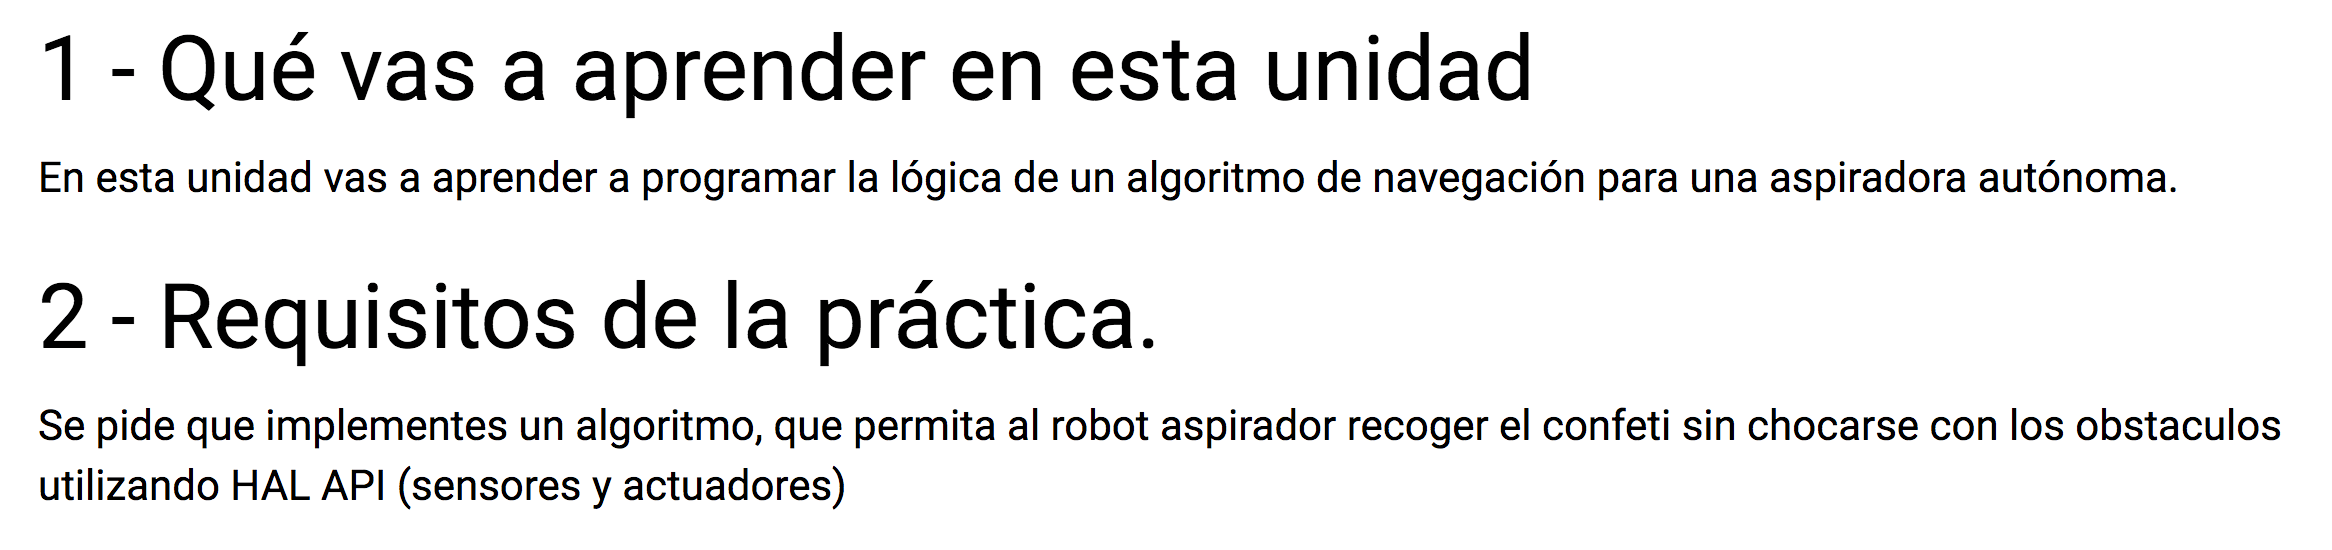
\includegraphics[width=0.8\textwidth, height=0.4\textwidth]{chapters/images/teoria2.png}
    \caption{Teoría}
    \label{fig:my_label}
\end{figure}
\begin{figure}[H]
    \centering
    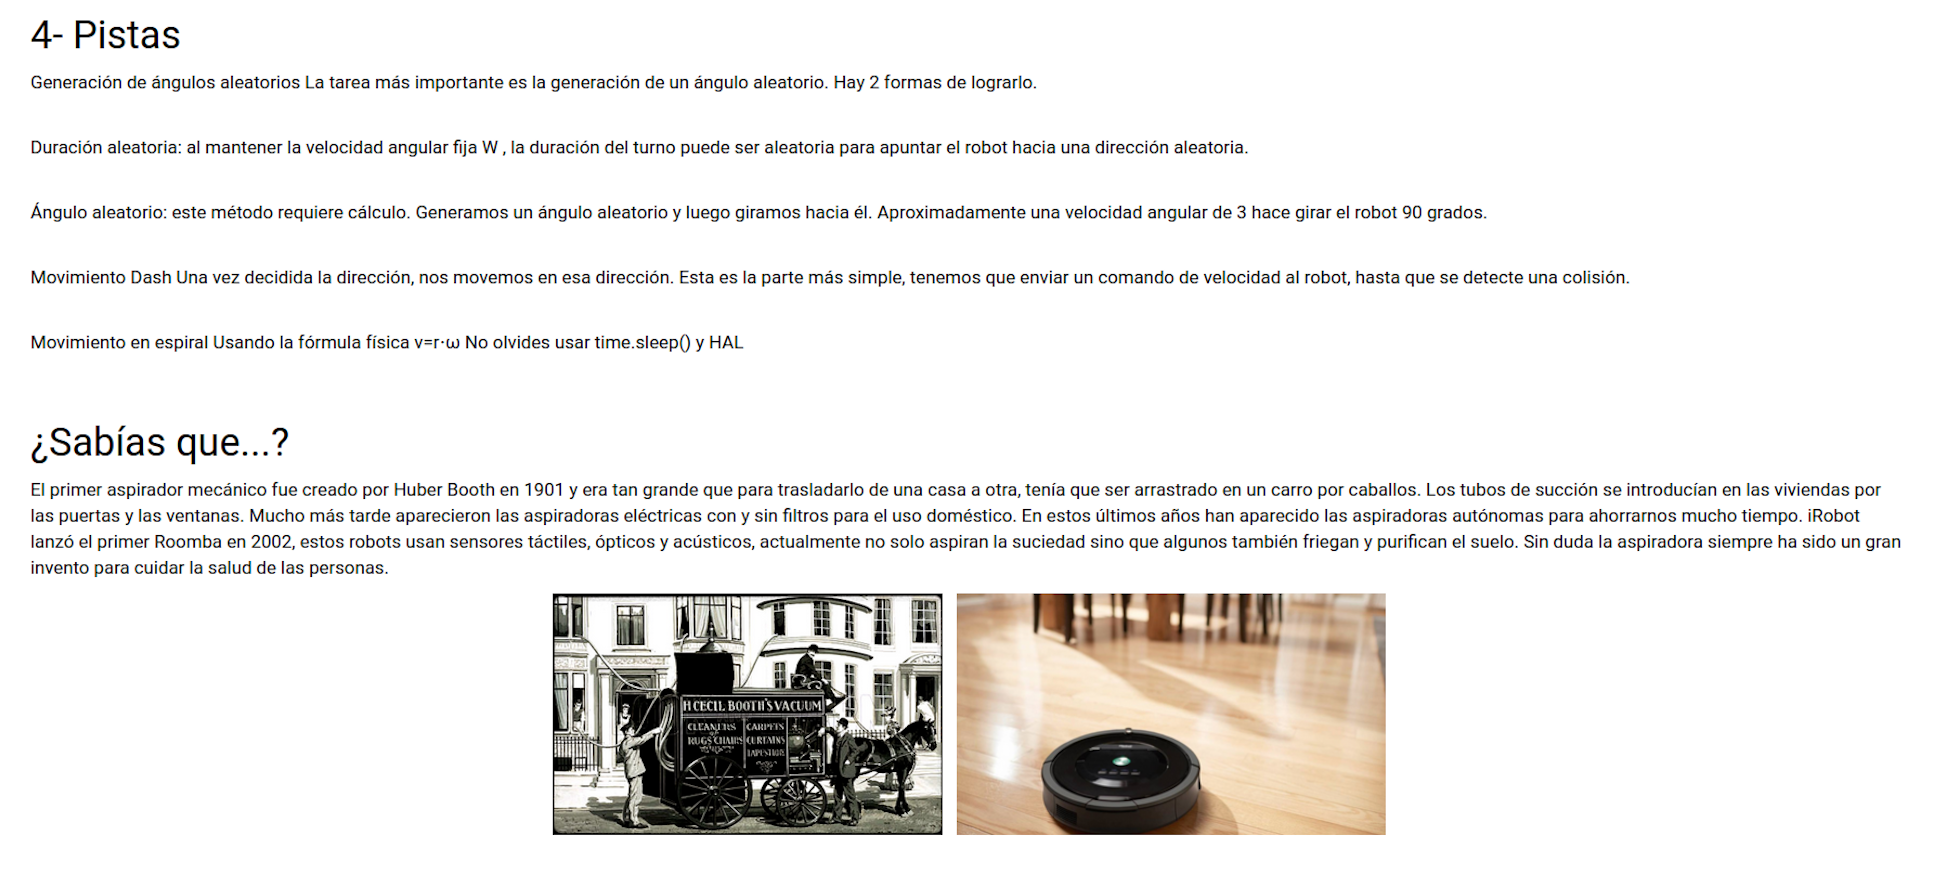
\includegraphics[width=0.8\textwidth, height=0.4\textwidth]{chapters/images/teoria3.png}
    \caption{Pistas y ¿sabías que.. ?}
    \label{fig:my_label}
\end{figure}


\section{Solución de referencia}

Hay muchas formas diferentes resolver este ejercicio, en este apartado se proponen dos soluciones en los dos lenguajes que nos proporciona Kibotics. En la Figura 5.9 se muestra una solución realizada en Scratch y en la Figura 5.10 una para Python.

\begin{figure}[H]
    \centering
    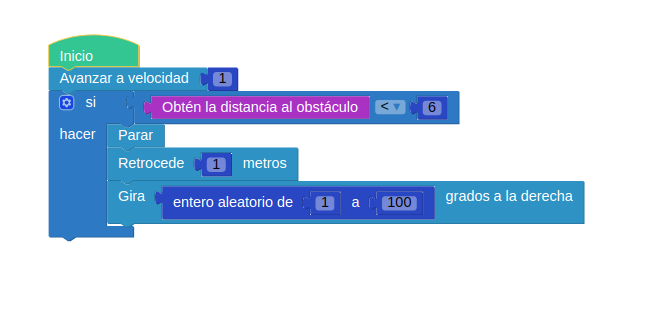
\includegraphics[width=0.8\textwidth, height=0.4\textwidth]{chapters/images/solucionroombascratch.png}
    \caption{Solución en Scratch }
    \label{fig:my_label}
\end{figure}
\begin{figure}[H]
    \centering
    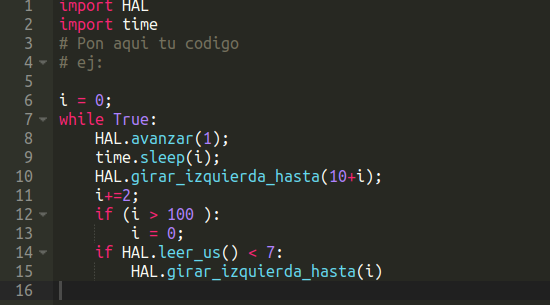
\includegraphics[width=0.8\textwidth, height=0.4\textwidth]{chapters/images/solucionroombapython.png}
    \caption{Solución en Python}
    \label{fig:my_label}
\end{figure}


Este ejercicio ya está disponible en la plataforma Kibotics. También se han realizado dos videos promocionales para presentar el nuevo ejercicio de la plataforma y como ejemplo para  los alumnos que vayan a realizar el ejercicio. Videos promocionales Python  \footnote{https://www.youtube.com/watch?v=5Q0TmwunYWY} y Scratch \footnote{https://www.youtube.com/watch?v=Twc9wsPFjaY}